\chapter{The Lanczos Iteration}
In the last three lectures we considered Krylov subspace iterations for nonhermitian matrix problems. We shall return to nonhermitian problems in Chapter 38, for there is more to this subject than Arnoldi and GMRES. But first, in this and the following two lectures, we specialize to the hermitian case, where a major simplification takes place.

\section{Three-Term Recurrence} 
 The Lanczos is the Arnoldi iteration specialized to the case where $ A $ is hermitian. Here, we assume $ A $ is real and symmetric. 

 For Arnoldi process in this special case, it follows from \eqref{eq: Arnoldi projection} that the Ritz matrix $ H_n $ is symmetric.  Hence, its eigenvalues the Ritz values or Lanczos estimates are also real. 

Since $ H_n $ is both symmetric and Hessenberg, it's tridiagonal. Hence, the $ (n+1) $-term recurrence at step $ n $ is replaced by 
\[
    Aq_n = h_{n-1, n} q_{n-1} + h_{nn} q_n + h_{n+1,n}q_{n+1}.  
\]
This is just a three-term recurrence. This means the inner loop of Arnoldi iteration (\autoref{Algo 33.1}), the limits 1 to $ n $ can be replaced by $ n-1 $ to $ n $.  Therefore, each step of the Lanczos iteration is much cheaper than the corresponding step of the Arnoldi iteration. 

The key equation for the tridiagonal property of $ H_n $ is that 
\[
    H_n = Q_n^*  A Q_n. 
\]
In fact, this is equal to say: 
\begin{equation}
\label{eq: element of H }
    h_{ij} = q_i^\top  A q_j. 
\end{equation}
This implies that $ h_{ij}=0$ for $ i>j+1 $, since $ Aq_j \in \langle q_1,q_2,\ldots ,q_{j+1} \rangle  $ and the Krylov vectors are orthogonal. Taking the transpose gives 
\[
    h_{ij} = q_j^\top A^\top q_i = q_jc^\top  A q_i.    
\]
Hence, $ h_{ij} = 0 $    for $ j>i+1 $. This simple argument leading to a three-term recurrence relation applies to arbitrary self-adjoint operator, not just to matrices.  


\section{ The Lanczos Iteration} 
Let $ \alpha _{n} = h_{nn} $ and $ \beta _{n} = h_{n+1,n} = h_{n,n+1} $. Then, $ H_{n} $ becomes 
\[
    T_{n} = \begin{bmatrix}[] 
        \alpha _{1} & \beta _{1} &  &  &   \\
        \beta _{1} & \alpha _2  & \beta _2  &  &   \\
         &  \beta _2& \alpha _3  &\ddots  &   \\
         &  & \ddots  &\ddots  & \beta _{n-1}   \\
         &  &  & \beta _{n-1}  & \alpha _n     \\
    \end{bmatrix} . 
\] 

\begin{algorithm}[H]
    \caption{Lanczos Iteration}
    \label{Algo 36.1}
    $ \beta _0 =0, q_0 = 0, b \text{ random }, q_1 = \frac{b}{\|b\|} $\; 
    \For{$n=1,2,3,...$}{
    $ v = Aq_n $\; 
    $ \alpha _n = q_n^\top v $\; 
    $ v = v - \beta _{n-1}q_{n-1} -\alpha _nq_n $\; 
    $ \beta _n = \|v\| $\; 
    $ q_{n+1} = \frac{v}{\beta _n} $\;
    }
\end{algorithm}
Each step consists of a matrix-vector multiplication, an inner product, and a couple of vector operations. If $ A $ has enough sparsity or other structure that matrix-vector products can be computed cheaply, then such an iteration can be applied without too much difficulty to problems of dimensions in the tens or hundreds of thousands. 


%────────────────────────────────────────
\begin{theorem}
[Properties of Lanczos iteration]
\label{thm: Properties of Lanczos iteration}
The matrices $Q_n$ of vectors $q_n$ generated by the Lanczos iteration are reduced $Q R$ factors of the Krylov matrix $ K_n $,
\begin{equation}
\label{eq: Lanczos QR}
K_n=Q_n R_n
\end{equation}
The tridiagonal matrices $T_n$ are the corresponding projections
\begin{equation}
\label{eq: Lanczos projection}
    T_n=Q_n^* A Q_n
\end{equation}
and the successive iterates are related by the formula
\begin{equation}
\label{eq: Lanczos iterate}
    A Q_n=Q_{n+1} \tilde{T}_n,
\end{equation}
which we can write in the form of a three-term recurrence at step $n$,
\begin{equation}
\label{eq: Lanczos three item}
    A q_n=\beta_{n-1} q_{n-1}+\alpha_n q_n+\beta_n q_{n+1} .
\end{equation}

As long as the Lanczos iteration does not break down (i.e., $K_n$ is of full rank n), the characteristic polynomial of $T_n$ is the unique polynomial $p^n \in$ $P^n$ that solves the Arnoldi/Lanczos approximation problem (34.3), i.e., that achieves
\begin{equation}
\label{eq: Lanczos approximation problem}
    \left\|p^n(A) b\right\|=\text { minimum }.
\end{equation}
\end{theorem}
%────────────────────────────────────────

\section{Lanczos and Electric Charge Distributions}

In practice, the Lanczos iteration is used to compute eigenvalues of large symmetric matrices just as the Arnoldi iteration is used for nonsymmetric matrices. At each step $n$, or at occasional steps, the eigenvalues of the growing tridiagonal matrix $T_n$ are determined by standard methods. Often some of these numbers are observed to converge geometrically to certain limits, which can then be expected to be eigenvalues of $A$.

As with the Arnoldi iteration, it is the outlying eigenvalues of $A$ that are most often obtained first.

\begin{itemize}
    \item If the eigenvalues of $A$ are more evenly spaced than Chebyshev points, then the Lanczos iteration will tend to find outliers.
\end{itemize}

Here is what this statement means. Suppose the $m$ eigenvalues $\left\{\lambda_j\right\}$ of $A$ are spread reasonably densely around an interval on the real axis. Since the Lanczos iteration is scale- and translation-invariant (Theorem~\ref{thm: Properties of Lanczos iteration}), we can assume without loss of generality that this interval is $[-1,1]$. The $m$ \textbf{Chebyshev points} in $[-1,1]$ are defined by the formula
\[
    x_j=\cos \theta_j, \quad \theta_j=\frac{\left(j-\frac{1}{2}\right) \pi}{m}, \quad 1 \leq j \leq m. 
\]
The exact definition is not important; what matters is that these points cluster quadratically near the endpoints, with the spacing between points $O\left(\mathrm{~m}^{-1}\right)$ in the interior and $O\left(\mathrm{~m}^{-2}\right)$ near $\pm 1$ . The rule of thumb asserts that if the eigenvalues $\left\{\lambda_j\right\}$ of $A$ are more evenly distributed than this-less clustered at the endpoints - then the Ritz values computed by a Lanczos iteration will tend to converge to the outlying eigenvalues first. In particular, an approximately uniform eigenvalue distribution will produce rapid convergence towards outliers. Conversely, if the eigenvalues of $A$ are more than quadratically clustered at the endpoints-a situation not so common in practice-then we can expect convergence to some of the ``inliers.''

These observations can be given a physical interpretation. Consider $m$ point charges free to move about the interval $[-1,1]$. Assume that the repulsive force between charges located at $x_j$ and $x_k$ is proportional to $\left|x_j-x_k\right|^{-1}$. (For electric charges in 3D the force would be $\left|x_j-x_k\right|^{-2}$, but this becomes $\left|x_j-x_k\right|^{-1}$ in 2D, where we can view each point as the intersection of an infinite line in 3D with the plane.) Let these charges distribute themselves in a minimal-energy equilibrium in $[-1,1]$. Then this minimal-energy distribution and the Chebyshev distribution are approximately the same, and in the limit $m \rightarrow \infty$, they both converge to a limiting continuous charge density distribution proportional to $\left(1-x^2\right)^{-1 / 2}$

Think of the eigenvalues of $A$ as point charges. If they are distributed approximately in a minimal-energy configuration in an interval, then the Lanczos iteration will be useless; there will be little convergence before step $n=m$. If the distribution is very different from this, however, then there is likely to be rapid convergence to some eigenvalues, namely, the eigenvalues in regions where there is "too little charge" in the sense that if the points were free to move, more would tend to cluster here. The rule of thumb can now be restated:

\begin{itemize}
    \item The Lanczos iteration tends to converge to eigenvalues in regions of "too little charge" for an equilibrium distribution.
\end{itemize}

\section{Example} 
Let $ A\in \RR^{203\times 203} $ and 
\[
    A = \diag(0, .01, .02, \ldots , 1.99, 2, 2.5, 3.0). 
\] 
Hence the spectrum of $ A $ consists of a dense collection of eigenvalues throughout $ [0,2] $ together with two outliers, $ 2.5 $ and $ 3.0 $. We carry out a Lanczos iteration beginning with a random starting vector $ q_1 $. 


Figure 35.1 shows the Ritz values and the associated Lanczos polynomial at step $n=9$. Seven of the Ritz values lie in [0,2], and the polynomial is uniformly small on that interval; the beginnings of a tendency for the Ritz values to cluster near the endpoints can be detected. The other two Ritz values lie near the eigenvalues at 2.5 and 3.0. The leading three Ritz values are
$$
1.93,2.48,2.999962 \text {. }
$$
Evidently we have little accuracy in the lower eigenvalues but five-digit accuracy in the leading one. A plot like this gives an idea of why outliers tend to be estimated accurately. The graph of $p(x)$ is so steep for $x \approx 3$ that if $p(3)$ is to be small, there must be a root of $p$ very close to 3 . This steepness of the graph is related to the presence of ``too little charge'' near this point. If the charges were free to move about $ [0,3] $ to minimize energy, more points would cluster near $ x=3 $ and $ p(x) $ would not be so steep there. 

At step 20 the leading three Ritz values are
$$
\text { 1.9906, } 2.499999999987, \quad 3.00000000000000 \text {. }
$$
Now we have about fifteen digits of accuracy in the leading eigenvalue and twelve digits in the second. A plot of $p(x)$ would be correspondingly steep near the points 2.5 and 3.0. Note that convergence to the third eigenvalue is also beginning to occur, a reflection of the fact that the eigenvalues in $[0,2]$ are distributed evenly rather than in a Chebyshev distribution.

%────────────────────────────────────────
\begin{figure}[H]
    \centering
    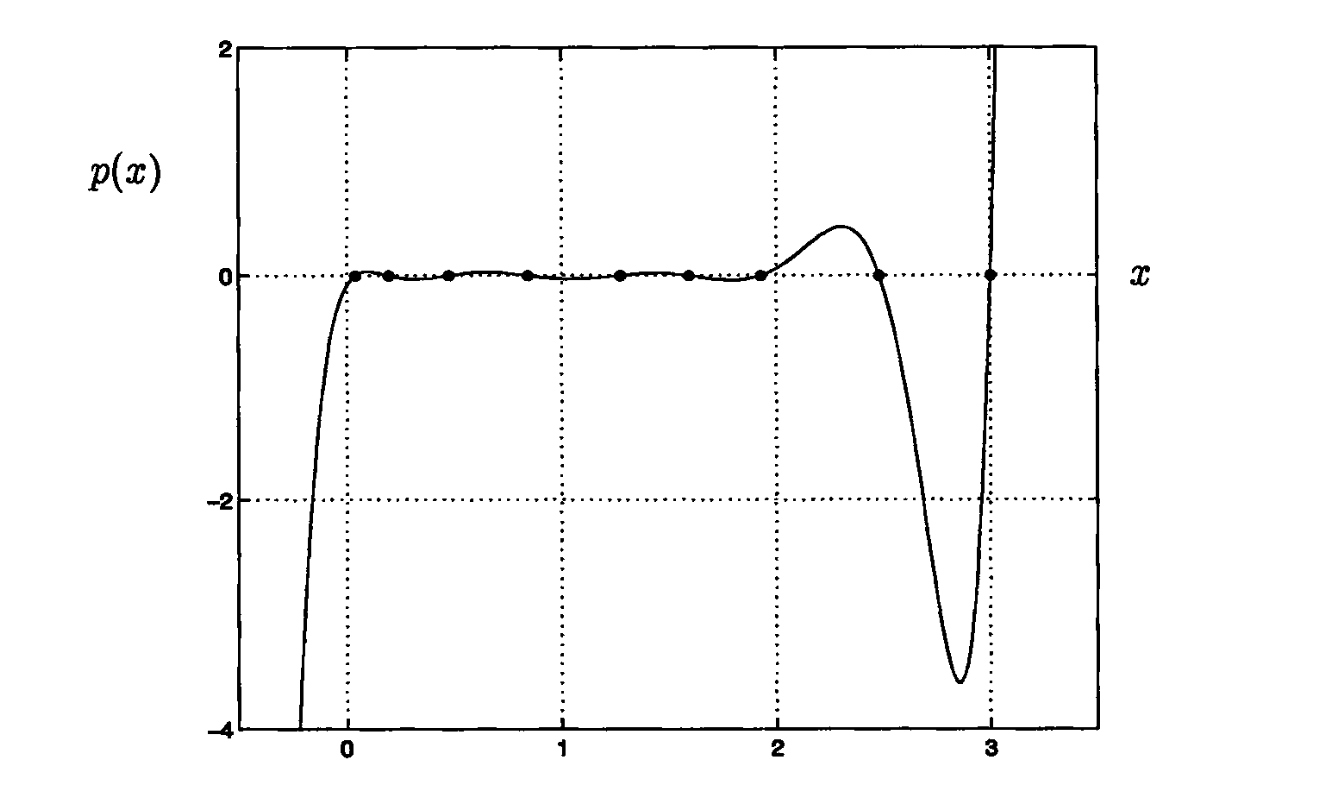
\includegraphics[width=0.8\textwidth]{figures/36-1.png}
    \caption{Plot of the Lanczos polynomial at step 9 of the Lanczos iteration for the matrix $ A $. The roots are the Ritz values or "Lanczos eigenvalue estimates." The polynomial is small throughout $[0,2] \cup\{2.5\} \cup\{3.0\}$. To achieve this, it must place one root near 2.5 and another very near 3.0.}
\end{figure}
%────────────────────────────────────────

%────────────────────────────────────────
\begin{figure}[H]
    \centering
    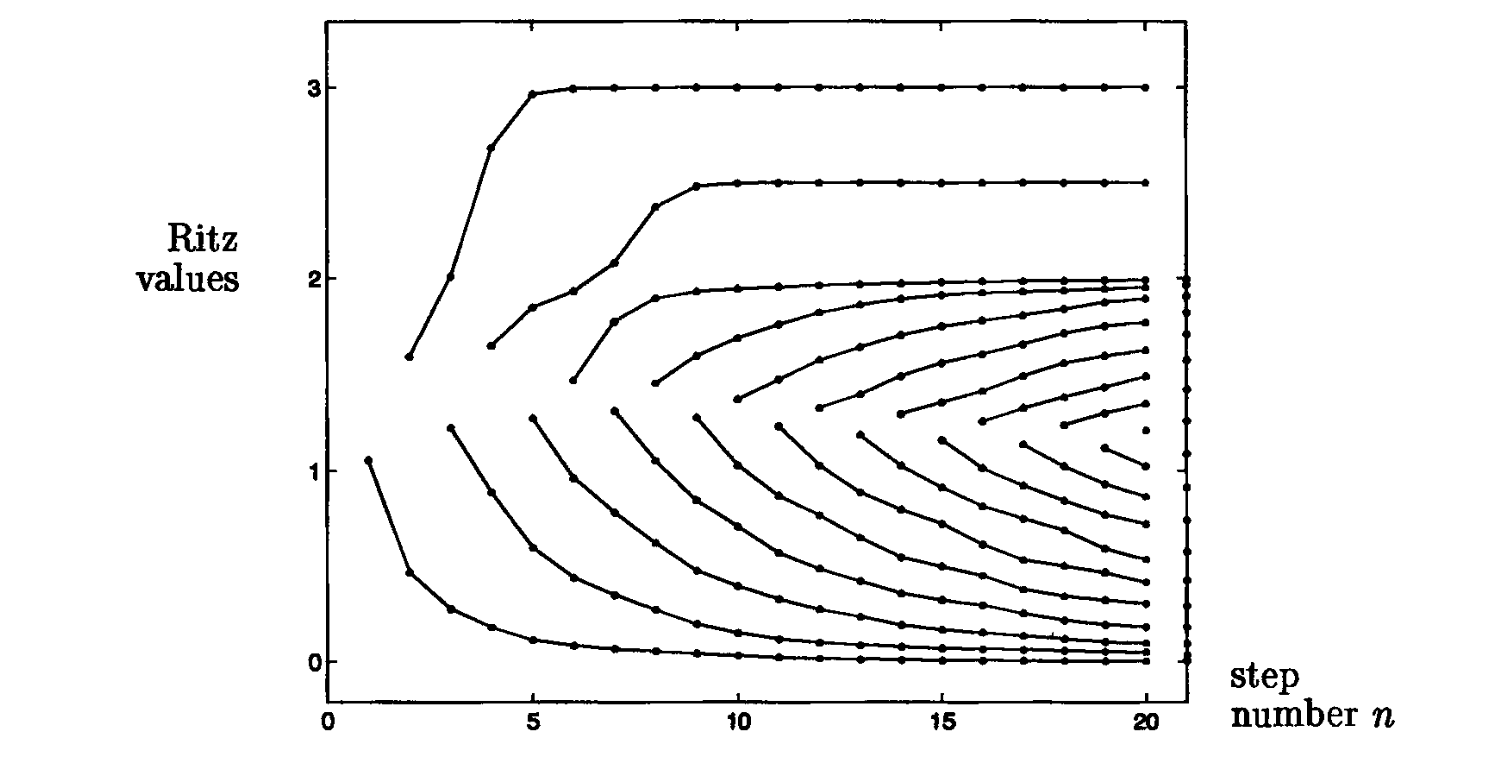
\includegraphics[width=0.8\textwidth]{figures/36-2.png}
    \caption{Ritz values for the first 20 steps of the Lanczos iteration applied to the same matrix. The convergence to the eigenvalues 2.5 and 3.0 is geometric. Little useful convergence to individual eigenvalues occurs in the $[0,2]$ part of the spectrum. Instead, the Ritz values in $[0,2]$ approximate Chebyshev points in that interval, marked by dots on the right-hand boundary.}
\end{figure}
%────────────────────────────────────────

An ``aerial view'' of the convergence process appears in Figure 36.2 , which shows the Ritz values for all steps from $n=1$ to $n=20$. Each vertical slice of this plot corresponds to the Ritz values at one iteration; the lines connecting the dots help the eye follow what is going on but have no precise meaning. The plot shows pronounced convergence to the leading eigenvalue after about $n=5$ and to the next one around $n=10$. In the interval $[0,2]$ containing the other eigenvalues, they show a density of Ritz values approximately proportional to $\left(1-x^2\right)^{-1 / 2}$, with very clear bunching at endpoints.

\section{Rounding Errors and ``Ghost'' Eigenvalues}
Rounding errors have a complex effect on the Lanczos iteration and, indeed, on all iterations of numerical linear algebra based on three-term recurrence relations. The source of the difficulty is easily identified. In an iteration based on an $n$-term recurrence relation, such as Arnoldi or GMRES, the vectors $q_1, q_2, q_3, \ldots$ are forced to be orthogonal by explicit Gram-Schmidt operations. Three-term recurrences like Lanczos and conjugate gradients, however, depend upon orthogonality of the vectors $\left\{q_j\right\}$ to arise "automatically" from a mathematical identity. In practice, such identities are not accurately preserved in the presence of rounding errors, and after a number of iterations, orthogonality is lost.

The loss of orthogonality in practical Lanczos iterations sounds wholly bad, but the situation is more subtle than that. As it happens, loss of orthogonality is connected closely with the convergence of Ritz values to eigenvalues of $A$. A great deal is known about this subject, though not as much as one might like; we shall not give details.

%────────────────────────────────────────
\begin{figure}[H]
    \centering
    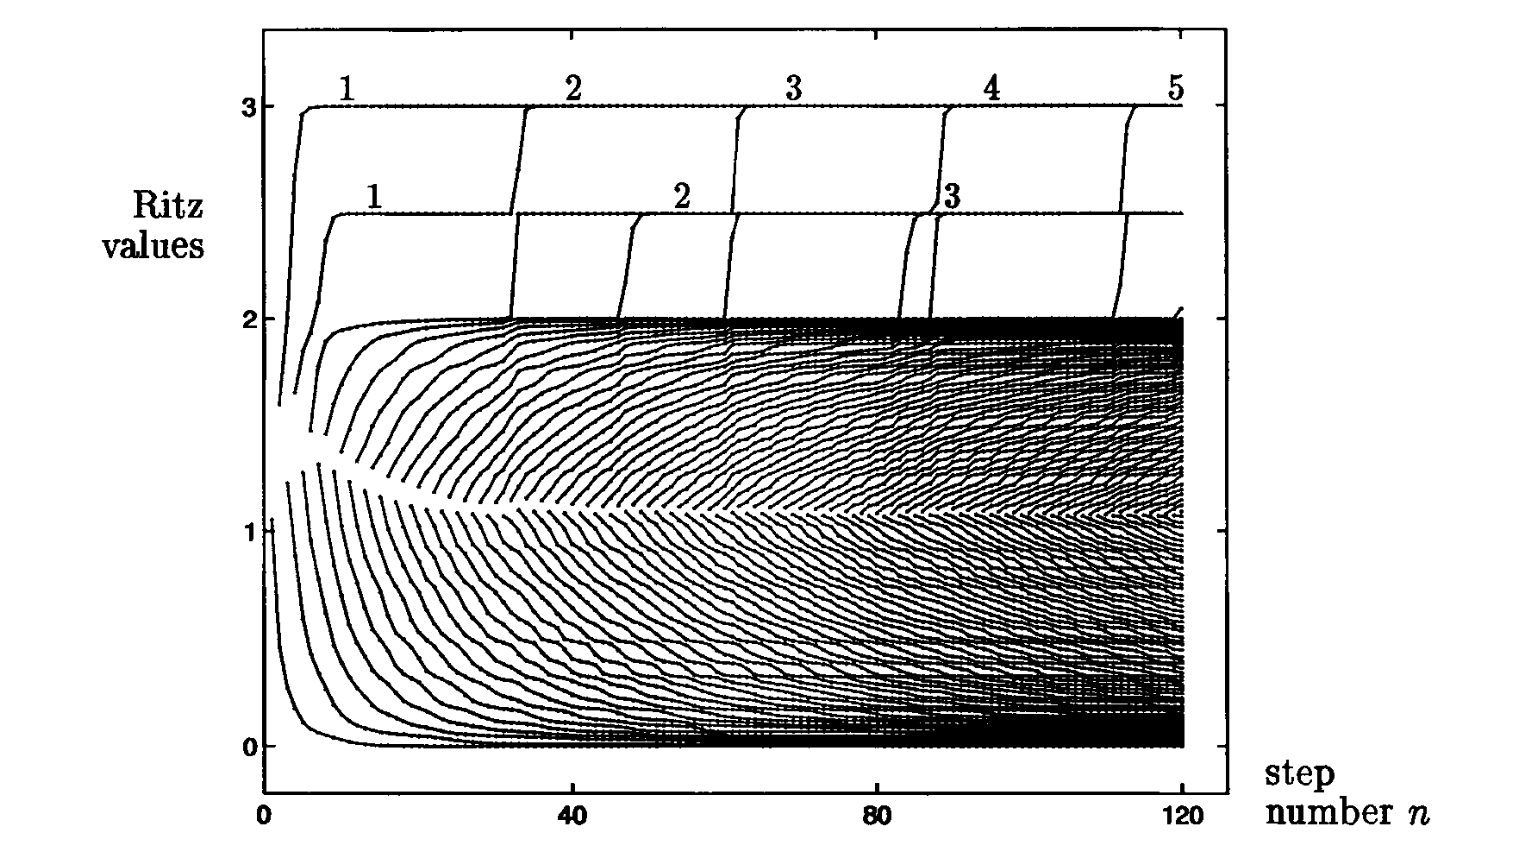
\includegraphics[width=0.8\textwidth]{figures/36-3.png}
    \caption{ Continuation to 120 steps of the Lanczos iteration. The numbers indicate multiplicities of the Ritz values. Note the appearance of four "ghost" copies of the eigenvalue 3.0 and two "ghost" copies of the eigenvalue 2.5 .}
\end{figure}
%────────────────────────────────────────
Because of complexities like these, no straightforward theorem is known to the effect that the Lanczos or conjugate gradient iterations is stable in the sense defined in this book. Nonetheless, these iterations are extraordinarily useful in practice. Figure 35.3 gives an idea of the way in which instability is often manifested in practice without preventing the iteration from being useful. The figure is a repetition of Figure 36.2 , but for 120 instead of 20 steps of the iteration. Everything looks as expected until around step 30, when a second copy of the eigenvalue 3.0 appears among the Ritz values. A third copy appears around step 60, a fourth copy around step 90, and so on. Meanwhile, additional copies of the eigenvalue 2.5 also appear around step 40 and 80 and (just beginning to be visible) 120 . These extra Ritz values are known as "ghost" eigenvalues, and they have nothing to do with the actual multiplicities of the corresponding eigenvalues of $A$.

A rigorous analysis of the phenomenon of ghost eigenvalues is complicated. Intuitive explanations, however, are not hard to devise. 
\begin{itemize}
    \item One idea is that in the presence of rounding errors, one should think of each eigenvalue of $A$ not as a point but as a small interval of size roughly $O\left(\epsilon_{\text {machine }}\|A\|\right)$; ghost eigenvalues arise from the need for $p(z)$ to be small not just at the exact eigenvalues but throughout these small intervals.
    \item Another, rather different explanation is that convergence of a Ritz value to an eigenvalue of $A$ annihilates the corresponding eigenvector component in the vector being operated upon; but in the presence of rounding errors, random noise must be expected to excite that component slightly again. After sufficiently many iterations, this previously annihilated component will have been amplified enough that another Ritz value is needed to annihilate it again-and then again, and again.
\end{itemize} 

Both of these explanations capture some of the truth about the behavior of the Lanczos iteration in floating point arithmetic. The second one has perhaps more quantitative accuracy.